\documentclass[]{article}
\usepackage{lmodern}
\usepackage{amssymb,amsmath}
\usepackage{ifxetex,ifluatex}
\usepackage{fixltx2e} % provides \textsubscript
\ifnum 0\ifxetex 1\fi\ifluatex 1\fi=0 % if pdftex
  \usepackage[T1]{fontenc}
  \usepackage[utf8]{inputenc}
\else % if luatex or xelatex
  \ifxetex
    \usepackage{mathspec}
  \else
    \usepackage{fontspec}
  \fi
  \defaultfontfeatures{Ligatures=TeX,Scale=MatchLowercase}
\fi
% use upquote if available, for straight quotes in verbatim environments
\IfFileExists{upquote.sty}{\usepackage{upquote}}{}
% use microtype if available
\IfFileExists{microtype.sty}{%
\usepackage{microtype}
\UseMicrotypeSet[protrusion]{basicmath} % disable protrusion for tt fonts
}{}
\usepackage[margin=2cm]{geometry}
\usepackage{hyperref}
\hypersetup{unicode=true,
            pdftitle={Statistical models},
            pdfauthor={Miao Cai miao.cai@slu.edu},
            pdfborder={0 0 0},
            breaklinks=true}
\urlstyle{same}  % don't use monospace font for urls
\usepackage{color}
\usepackage{fancyvrb}
\newcommand{\VerbBar}{|}
\newcommand{\VERB}{\Verb[commandchars=\\\{\}]}
\DefineVerbatimEnvironment{Highlighting}{Verbatim}{commandchars=\\\{\}}
% Add ',fontsize=\small' for more characters per line
\usepackage{framed}
\definecolor{shadecolor}{RGB}{248,248,248}
\newenvironment{Shaded}{\begin{snugshade}}{\end{snugshade}}
\newcommand{\AlertTok}[1]{\textcolor[rgb]{0.94,0.16,0.16}{#1}}
\newcommand{\AnnotationTok}[1]{\textcolor[rgb]{0.56,0.35,0.01}{\textbf{\textit{#1}}}}
\newcommand{\AttributeTok}[1]{\textcolor[rgb]{0.77,0.63,0.00}{#1}}
\newcommand{\BaseNTok}[1]{\textcolor[rgb]{0.00,0.00,0.81}{#1}}
\newcommand{\BuiltInTok}[1]{#1}
\newcommand{\CharTok}[1]{\textcolor[rgb]{0.31,0.60,0.02}{#1}}
\newcommand{\CommentTok}[1]{\textcolor[rgb]{0.56,0.35,0.01}{\textit{#1}}}
\newcommand{\CommentVarTok}[1]{\textcolor[rgb]{0.56,0.35,0.01}{\textbf{\textit{#1}}}}
\newcommand{\ConstantTok}[1]{\textcolor[rgb]{0.00,0.00,0.00}{#1}}
\newcommand{\ControlFlowTok}[1]{\textcolor[rgb]{0.13,0.29,0.53}{\textbf{#1}}}
\newcommand{\DataTypeTok}[1]{\textcolor[rgb]{0.13,0.29,0.53}{#1}}
\newcommand{\DecValTok}[1]{\textcolor[rgb]{0.00,0.00,0.81}{#1}}
\newcommand{\DocumentationTok}[1]{\textcolor[rgb]{0.56,0.35,0.01}{\textbf{\textit{#1}}}}
\newcommand{\ErrorTok}[1]{\textcolor[rgb]{0.64,0.00,0.00}{\textbf{#1}}}
\newcommand{\ExtensionTok}[1]{#1}
\newcommand{\FloatTok}[1]{\textcolor[rgb]{0.00,0.00,0.81}{#1}}
\newcommand{\FunctionTok}[1]{\textcolor[rgb]{0.00,0.00,0.00}{#1}}
\newcommand{\ImportTok}[1]{#1}
\newcommand{\InformationTok}[1]{\textcolor[rgb]{0.56,0.35,0.01}{\textbf{\textit{#1}}}}
\newcommand{\KeywordTok}[1]{\textcolor[rgb]{0.13,0.29,0.53}{\textbf{#1}}}
\newcommand{\NormalTok}[1]{#1}
\newcommand{\OperatorTok}[1]{\textcolor[rgb]{0.81,0.36,0.00}{\textbf{#1}}}
\newcommand{\OtherTok}[1]{\textcolor[rgb]{0.56,0.35,0.01}{#1}}
\newcommand{\PreprocessorTok}[1]{\textcolor[rgb]{0.56,0.35,0.01}{\textit{#1}}}
\newcommand{\RegionMarkerTok}[1]{#1}
\newcommand{\SpecialCharTok}[1]{\textcolor[rgb]{0.00,0.00,0.00}{#1}}
\newcommand{\SpecialStringTok}[1]{\textcolor[rgb]{0.31,0.60,0.02}{#1}}
\newcommand{\StringTok}[1]{\textcolor[rgb]{0.31,0.60,0.02}{#1}}
\newcommand{\VariableTok}[1]{\textcolor[rgb]{0.00,0.00,0.00}{#1}}
\newcommand{\VerbatimStringTok}[1]{\textcolor[rgb]{0.31,0.60,0.02}{#1}}
\newcommand{\WarningTok}[1]{\textcolor[rgb]{0.56,0.35,0.01}{\textbf{\textit{#1}}}}
\usepackage{graphicx,grffile}
\makeatletter
\def\maxwidth{\ifdim\Gin@nat@width>\linewidth\linewidth\else\Gin@nat@width\fi}
\def\maxheight{\ifdim\Gin@nat@height>\textheight\textheight\else\Gin@nat@height\fi}
\makeatother
% Scale images if necessary, so that they will not overflow the page
% margins by default, and it is still possible to overwrite the defaults
% using explicit options in \includegraphics[width, height, ...]{}
\setkeys{Gin}{width=\maxwidth,height=\maxheight,keepaspectratio}
\IfFileExists{parskip.sty}{%
\usepackage{parskip}
}{% else
\setlength{\parindent}{0pt}
\setlength{\parskip}{6pt plus 2pt minus 1pt}
}
\setlength{\emergencystretch}{3em}  % prevent overfull lines
\providecommand{\tightlist}{%
  \setlength{\itemsep}{0pt}\setlength{\parskip}{0pt}}
\setcounter{secnumdepth}{5}
% Redefines (sub)paragraphs to behave more like sections
\ifx\paragraph\undefined\else
\let\oldparagraph\paragraph
\renewcommand{\paragraph}[1]{\oldparagraph{#1}\mbox{}}
\fi
\ifx\subparagraph\undefined\else
\let\oldsubparagraph\subparagraph
\renewcommand{\subparagraph}[1]{\oldsubparagraph{#1}\mbox{}}
\fi

%%% Use protect on footnotes to avoid problems with footnotes in titles
\let\rmarkdownfootnote\footnote%
\def\footnote{\protect\rmarkdownfootnote}

%%% Change title format to be more compact
\usepackage{titling}

% Create subtitle command for use in maketitle
\providecommand{\subtitle}[1]{
  \posttitle{
    \begin{center}\large#1\end{center}
    }
}

\setlength{\droptitle}{-2em}

  \title{Statistical models}
    \pretitle{\vspace{\droptitle}\centering\huge}
  \posttitle{\par}
    \author{Miao Cai \href{mailto:miao.cai@slu.edu}{\nolinkurl{miao.cai@slu.edu}}}
    \preauthor{\centering\large\emph}
  \postauthor{\par}
      \predate{\centering\large\emph}
  \postdate{\par}
    \date{8/8/2019}

\usepackage{float}
\usepackage{dcolumn}
\usepackage{booktabs}

\begin{document}
\maketitle

\hypertarget{logit}{%
\section{Logit}\label{logit}}

\begin{Shaded}
\begin{Highlighting}[]
\NormalTok{pacman}\OperatorTok{::}\KeywordTok{p_load}\NormalTok{(data.table, rstanarm)}
\NormalTok{agg30 =}\StringTok{ }\KeywordTok{fread}\NormalTok{(}\StringTok{"data/31-analyses_30_minute_intervals.csv"}\NormalTok{)}
\end{Highlighting}
\end{Shaded}

\begin{Shaded}
\begin{Highlighting}[]
\NormalTok{fitlogit =}\StringTok{ }\KeywordTok{stan_glmer}\NormalTok{(SCE_binary }\OperatorTok{~}\StringTok{ }\DecValTok{1} \OperatorTok{+}\StringTok{ }\NormalTok{cum_drive }\OperatorTok{+}\StringTok{ }\NormalTok{age }\OperatorTok{+}\StringTok{ }
\StringTok{                        }\NormalTok{precip_intensity }\OperatorTok{+}\StringTok{ }\NormalTok{precip_probability }\OperatorTok{+}\StringTok{ }
\StringTok{                        }\NormalTok{wind_speed }\OperatorTok{+}\StringTok{ }\NormalTok{visibility }\OperatorTok{+}\StringTok{ }
\StringTok{                        }\NormalTok{speed_limit }\OperatorTok{+}\StringTok{ }\NormalTok{num_lanes }\OperatorTok{+}\StringTok{ }\NormalTok{interval_time }\OperatorTok{+}\StringTok{ }
\StringTok{                        }\NormalTok{(}\DecValTok{1} \OperatorTok{+}\StringTok{ }\NormalTok{cum_drive}\OperatorTok{|}\NormalTok{driver), }\DataTypeTok{data =} \KeywordTok{as.data.frame}\NormalTok{(agg30), }
                      \DataTypeTok{family =} \KeywordTok{binomial}\NormalTok{(}\DataTypeTok{link =} \StringTok{"logit"}\NormalTok{), }
                      \DataTypeTok{QR=}\OtherTok{TRUE}\NormalTok{, }\DataTypeTok{chains =} \DecValTok{4}\NormalTok{, }\DataTypeTok{iter =} \DecValTok{2000}\NormalTok{)}
\KeywordTok{saveRDS}\NormalTok{(fitlogit, }\StringTok{"fit/logit_fit.rds"}\NormalTok{)}

\NormalTok{broom}\OperatorTok{::}\KeywordTok{tidy}\NormalTok{(fitlogit, }\DataTypeTok{intervals =} \OtherTok{TRUE}\NormalTok{, }\DataTypeTok{prob =} \FloatTok{0.5}\NormalTok{)}
\NormalTok{broom}\OperatorTok{::}\KeywordTok{tidy}\NormalTok{(fitlogit, }\DataTypeTok{parameters =} \StringTok{"hierarchical"}\NormalTok{)}
\NormalTok{broom}\OperatorTok{::}\KeywordTok{tidy}\NormalTok{(fitlogit, }\DataTypeTok{parameters =} \StringTok{"varying"}\NormalTok{)}
\end{Highlighting}
\end{Shaded}

\hypertarget{poisson}{%
\section{Poisson}\label{poisson}}

\begin{Shaded}
\begin{Highlighting}[]
\NormalTok{fitpoisson =}\StringTok{ }\KeywordTok{stan_glmer}\NormalTok{(n_SCE }\OperatorTok{~}\StringTok{ }\DecValTok{1} \OperatorTok{+}\StringTok{ }\NormalTok{cum_drive }\OperatorTok{+}\StringTok{ }\NormalTok{age }\OperatorTok{+}\StringTok{ }
\StringTok{                          }\NormalTok{precip_intensity }\OperatorTok{+}\StringTok{ }\NormalTok{precip_probability }\OperatorTok{+}\StringTok{ }
\StringTok{                        }\NormalTok{wind_speed }\OperatorTok{+}\StringTok{ }\NormalTok{visibility }\OperatorTok{+}\StringTok{ }\NormalTok{speed_limit }\OperatorTok{+}\StringTok{ }\NormalTok{num_lanes }\OperatorTok{+}\StringTok{ }
\StringTok{                        }\NormalTok{(}\DecValTok{1} \OperatorTok{+}\StringTok{ }\NormalTok{cum_drive}\OperatorTok{|}\NormalTok{driver), }
                        \DataTypeTok{offset =} \KeywordTok{log}\NormalTok{(interval_time),}
                      \DataTypeTok{data =} \KeywordTok{as.data.frame}\NormalTok{(agg30), }
                      \DataTypeTok{family =} \StringTok{"poisson"}\NormalTok{, }
                      \DataTypeTok{QR=}\OtherTok{TRUE}\NormalTok{, }\DataTypeTok{chains =} \DecValTok{4}\NormalTok{, }\DataTypeTok{iter =} \DecValTok{2000}\NormalTok{)}
\KeywordTok{saveRDS}\NormalTok{(fitpoisson, }\StringTok{"fit/poisson_fit.rds"}\NormalTok{)}

\NormalTok{broom}\OperatorTok{::}\KeywordTok{tidy}\NormalTok{(fitpoisson, }\DataTypeTok{intervals =} \OtherTok{TRUE}\NormalTok{, }\DataTypeTok{prob =} \FloatTok{0.5}\NormalTok{)}
\NormalTok{broom}\OperatorTok{::}\KeywordTok{tidy}\NormalTok{(fitpoisson, }\DataTypeTok{parameters =} \StringTok{"hierarchical"}\NormalTok{)}
\NormalTok{broom}\OperatorTok{::}\KeywordTok{tidy}\NormalTok{(fitpoisson, }\DataTypeTok{parameters =} \StringTok{"varying"}\NormalTok{)}
\end{Highlighting}
\end{Shaded}

\hypertarget{nhpp}{%
\section{NHPP}\label{nhpp}}

\hypertarget{read-data}{%
\subsection{Read data}\label{read-data}}

\begin{Shaded}
\begin{Highlighting}[]
\NormalTok{pacman}\OperatorTok{::}\KeywordTok{p_load}\NormalTok{(dplyr, ggplot2, rstan, data.table, lubridate)}
\NormalTok{shif =}\StringTok{ }\NormalTok{data.table}\OperatorTok{::}\KeywordTok{fread}\NormalTok{(}\StringTok{"data/32-analyses_shifts.csv"}\NormalTok{)}
\NormalTok{event_tab =}\StringTok{ }\NormalTok{data.table}\OperatorTok{::}\KeywordTok{fread}\NormalTok{(}\StringTok{"data/33-analyses_events.csv"}\NormalTok{) }\OperatorTok\StringTok{ }
\StringTok{  }\NormalTok{.[,shift_id }\OperatorTok{:}\ErrorTok{=}\StringTok{ }\KeywordTok{as.integer}\NormalTok{(}\KeywordTok{as.factor}\NormalTok{(}\KeywordTok{paste0}\NormalTok{(driver, shift_ID)))]}
\end{Highlighting}
\end{Shaded}

\hypertarget{stan-estimation}{%
\subsection{Stan estimation}\label{stan-estimation}}

\begin{Shaded}
\begin{Highlighting}[]
\NormalTok{standat =}\StringTok{ }\KeywordTok{list}\NormalTok{(}
  \DataTypeTok{N =}\NormalTok{ shif[,}\KeywordTok{sum}\NormalTok{(n_SCE)],}
  \DataTypeTok{K =} \KeywordTok{ncol}\NormalTok{(shif[,age}\OperatorTok{:}\NormalTok{num_lanes]),}
  \DataTypeTok{S =}\NormalTok{ shif[,.N],}
  \DataTypeTok{D =}\NormalTok{ shif[,}\KeywordTok{length}\NormalTok{(}\KeywordTok{unique}\NormalTok{(driver))],}
  \DataTypeTok{id =}\NormalTok{ shif[,}\KeywordTok{as.integer}\NormalTok{(}\KeywordTok{as.factor}\NormalTok{(driver))],}
  \DataTypeTok{tau =}\NormalTok{ shif[,shift_length}\OperatorTok{/}\DecValTok{60}\NormalTok{],}
  \DataTypeTok{event_time =}\NormalTok{ event_tab[,time2event}\OperatorTok{/}\DecValTok{60}\NormalTok{],}
  \DataTypeTok{group_size =}\NormalTok{ shif[,n_SCE],}
  \DataTypeTok{X_predictors =} \KeywordTok{as.matrix}\NormalTok{(shif[,age}\OperatorTok{:}\NormalTok{num_lanes])}
\NormalTok{)}

\NormalTok{fit =}\StringTok{ }\KeywordTok{stan}\NormalTok{(}\StringTok{"stan/nhpp_non_center.stan"}\NormalTok{,}
         \DataTypeTok{chains =} \DecValTok{4}\NormalTok{, }\DataTypeTok{iter =} \DecValTok{2000}\NormalTok{, }\DataTypeTok{data =}\NormalTok{ standat, }
         \DataTypeTok{cores =} \DecValTok{4}\NormalTok{, }\DataTypeTok{seed =} \DecValTok{123}\NormalTok{)}\CommentTok{#, init_r = .5}

\KeywordTok{saveRDS}\NormalTok{(fit, }\StringTok{"fit/nhpp_fit_non_center.rds"}\NormalTok{)}
\end{Highlighting}
\end{Shaded}

\begin{Shaded}
\begin{Highlighting}[]
\NormalTok{fitnhpp =}\StringTok{ }\KeywordTok{readRDS}\NormalTok{(}\StringTok{"fit/nhpp_fit_non_center.rds"}\NormalTok{)}
\NormalTok{tracep =}\StringTok{ }\NormalTok{rstan}\OperatorTok{::}\KeywordTok{traceplot}\NormalTok{(fitnhpp, }\StringTok{"beta"}\NormalTok{)}
\KeywordTok{ggsave}\NormalTok{(}\StringTok{"figs/traceplot_beta.png"}\NormalTok{, }\DataTypeTok{width =} \DecValTok{10}\NormalTok{, }\DataTypeTok{height =} \FloatTok{6.18}\NormalTok{, }\DataTypeTok{dpi =} \DecValTok{300}\NormalTok{)}
\NormalTok{tracep}
\end{Highlighting}
\end{Shaded}

\begin{figure}
\centering
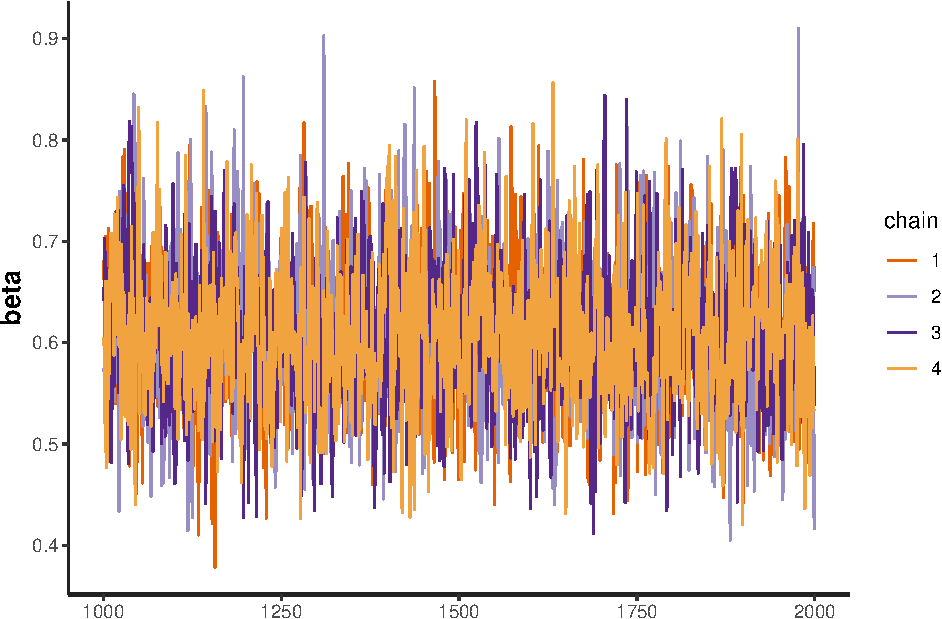
\includegraphics{02_Stats_models_files/figure-latex/exampletrace-1.pdf}
\caption{Example trace plot for shape parameter \(\beta\) in NHPP}
\end{figure}

\hypertarget{arrow-plot}{%
\subsection{Arrow plot}\label{arrow-plot}}

\begin{Shaded}
\begin{Highlighting}[]
\NormalTok{start_end_dat =}\StringTok{ }\NormalTok{event_tab }\OperatorTok\StringTok{ }
\StringTok{  }\NormalTok{.[,.(}\DataTypeTok{start_time =} \DecValTok{0}\NormalTok{, }\DataTypeTok{end_time =}\NormalTok{ shift_length),}
\NormalTok{    shift_id]}

\NormalTok{p =}\StringTok{ }\NormalTok{event_tab }\OperatorTok\StringTok{ }
\StringTok{    }\KeywordTok{ggplot}\NormalTok{(}\KeywordTok{aes}\NormalTok{(}\DataTypeTok{x =}\NormalTok{ time2event, }\DataTypeTok{y =}\NormalTok{ shift_id)) }\OperatorTok{+}\StringTok{ }
\StringTok{    }\KeywordTok{geom_point}\NormalTok{(}\DataTypeTok{alpha =} \FloatTok{0.8}\NormalTok{, }\DataTypeTok{shape =} \DecValTok{4}\NormalTok{, }\DataTypeTok{color =} \StringTok{'red'}\NormalTok{, }\DataTypeTok{size =} \DecValTok{4}\NormalTok{) }\OperatorTok{+}\StringTok{ }
\StringTok{    }\KeywordTok{scale_y_continuous}\NormalTok{(}\StringTok{"shift ID"}\NormalTok{, }
                       \DataTypeTok{labels =} \KeywordTok{as.character}\NormalTok{(event_tab}\OperatorTok{$}\NormalTok{shift_id), }
                       \DataTypeTok{breaks =}\NormalTok{ event_tab}\OperatorTok{$}\NormalTok{shift_id)}\OperatorTok{+}
\StringTok{    }\KeywordTok{xlab}\NormalTok{(}\StringTok{'Time to event (minutes)'}\NormalTok{) }\OperatorTok{+}\StringTok{ }
\StringTok{    }\KeywordTok{geom_segment}\NormalTok{(}\DataTypeTok{data =}\NormalTok{ start_end_dat,}
                 \KeywordTok{aes}\NormalTok{(}\DataTypeTok{x =}\NormalTok{ start_time, }\DataTypeTok{xend =}\NormalTok{ end_time, }
                     \DataTypeTok{y =}\NormalTok{ shift_id, }\DataTypeTok{yend =}\NormalTok{ shift_id),}
                 \DataTypeTok{lineend =} \StringTok{'butt'}\NormalTok{,}
                 \DataTypeTok{arrow =} \KeywordTok{arrow}\NormalTok{(}\DataTypeTok{length =} \KeywordTok{unit}\NormalTok{(}\FloatTok{0.2}\NormalTok{, }\StringTok{"cm"}\NormalTok{))) }\OperatorTok{+}\StringTok{ }
\StringTok{  }\KeywordTok{labs}\NormalTok{(}\DataTypeTok{x =} \StringTok{"Time (hours)"}\NormalTok{)}\OperatorTok{+}
\StringTok{  }\KeywordTok{theme_test}\NormalTok{()}

\KeywordTok{ggsave}\NormalTok{(}\StringTok{"figs/t2events_arrow_plot.png"}\NormalTok{, p, }\DataTypeTok{width =} \DecValTok{6}\NormalTok{, }\DataTypeTok{height =} \DecValTok{6}\NormalTok{, }\DataTypeTok{dpi =} \DecValTok{300}\NormalTok{)}
\end{Highlighting}
\end{Shaded}

\begin{Shaded}
\begin{Highlighting}[]
\NormalTok{knitr}\OperatorTok{::}\KeywordTok{include_graphics}\NormalTok{(}\StringTok{"figs/t2events_arrow_plot.png"}\NormalTok{)}
\end{Highlighting}
\end{Shaded}

\begin{figure}
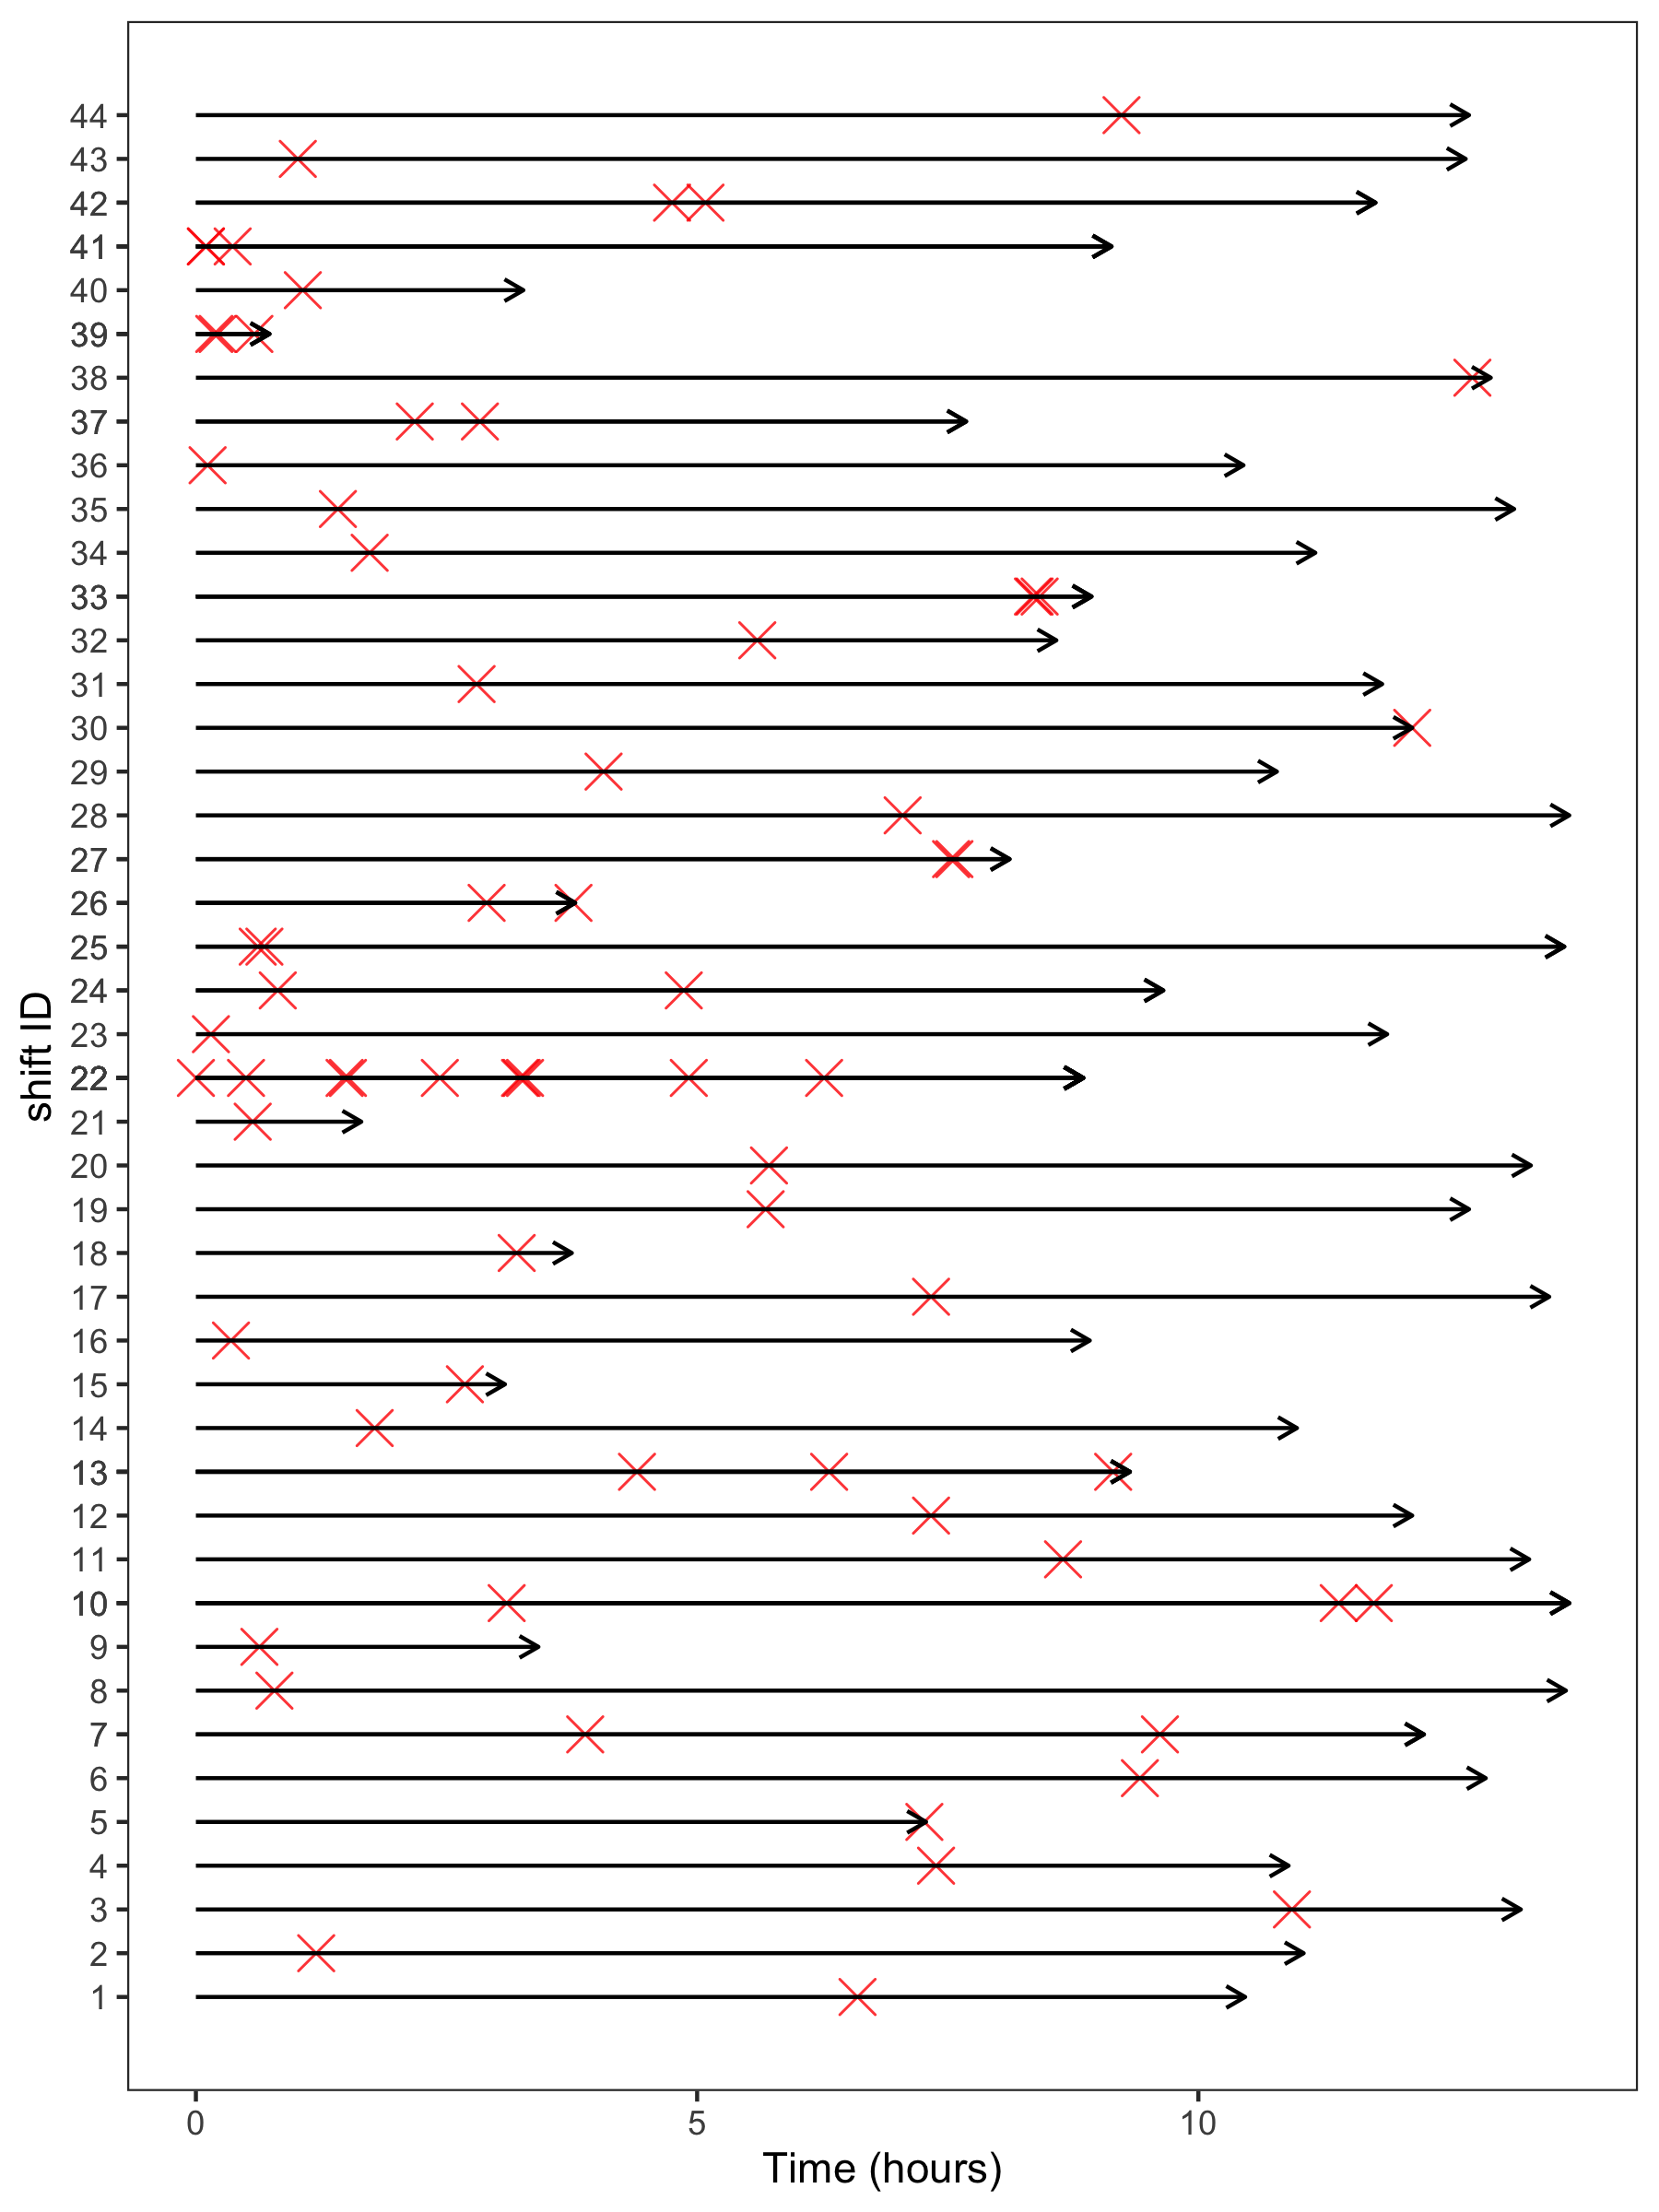
\includegraphics[width=25in]{figs/t2events_arrow_plot} \caption{Arrow plot of time of SCEs in each shift}\label{fig:unnamed-chunk-6}
\end{figure}


\end{document}
